\section{物体に作用する力とつり合い}

\subsection{力のつり合いと運動の法則}

物体に力が働く（=作用する）と，物体は変形したり，その運動状態が変化したりする．
すなわち，{\bf 物体の状態はその物体に作用している力によって定まる．}
よって，物体に作用する力を把握することが重要である．

力は加える向きと，加える大きさの2つを持つので，$\overrightarrow{f}や\overrightarrow{F}$などとベクトルを用いて表す．
この表し方を用いて，ある物体に作用する2つの力をベクトル合成により1つにまとめたり（合力），もしくは1つの力を成分分解により2つの力に分解したりすることができる．


\begin{figure}[h]
\begin{center}

\includegraphics[width=100mm]{text_p14_fig1.png}
\end{center}
\end{figure}

物体に作用するすべての力の合力が$\overrightarrow{0}$であるとき，{\bf 力がつり合っている}という．
このとき，静止している物体は静止し続け，動いている物体はその速度を維持し続けて等速度直線運動を行う．
これを{\bf 慣性の法則（運動の第一法則）}という．
この慣性の法則をはじめ，運動に関する性質をまとめたものを{\bf ニュートンの運動の法則}という．

\begin{matome}{運動の法則}
 $\hspace{10mm}{\bf 第一法則　慣性の法則}\\
 \hspace{15mm} 物体に作用する力の合力が\overrightarrow{0}{\rm [N]}となる場合，物体は静止または等速度運動を行う．\\
 \hspace{10mm}{\bf 第二法則　運動方程式}\\
 \hspace{15mm} 物体に作用する力の合力を\overrightarrow{F}{\rm [N]}とすれば，物体は加速度運動を行い，質量をm{\rm [kg]}，\\ \hspace{15mm}加速度を\overrightarrow{a} {\rm [m/s^2]}とすると，m\overrightarrow{a}=\overrightarrow{F}が成立する．\\
  \hspace{10mm}{\bf 第三法則　作用反作用の法則}\\
 \hspace{15mm} 物体Aが物体Bに力を及ぼすとき，物体Aは物体Bから等大逆向きの力を受ける．$
\end{matome}

\newpage
\subsection{力学問題の基本的な解法}

以上の運動の法則に基づいて，力学の問題は以下の手順に従って解くことが基本となる．
\begin{matome}{力学問題の基本的な解法}
 $\hspace{10mm}{\bf \MARU{1}　各物体に作用している力を描き出す}\\
 \hspace{15mm} \underline{ポイント}　・場の力以外は接触しているものからしか力を受けない．\\
 \hspace{32mm} ・複数物体がある場合は各物体ごとに別々に描くと良い．\\
 \hspace{10mm}{\bf \MARU{2}　各方向ごとに運動方程式または力のつり合いを立てる}\\
 \hspace{15mm} \underline{ポイント}　・必要に応じてx軸，y軸を設定し，力をそれぞれの成分に分解する．\\
 \hspace{32mm} ・極力分解する力，または加速度が少なくなる方向を選ぶ．\\ 
 \hspace{10mm}{\bf \MARU{3}　式を連立して未知数について解く}\\
 \hspace{15mm} \underline{ポイント}　・どれが未知数なのかを意識して式変形していく．\\
 \hspace{32mm} ・未知数の数に対して式の数が足りない場合は，束縛条件やまだ使っていない\\\hspace{33mm}問題文中に与えられている条件がないかを探してみる．\\
  \hspace{10mm}{\bf \MARU{4}　設問に応じて運動を解析する}\\
 \hspace{15mm} \underline{ポイント}　・等加速度運動となる場合，v=v_0+at,\hspace{1mm}x=x_0+v_0t+\dfrac{1}{2}at^2,\hspace{1mm}v^2-v_0^2=2a(x-x_0)\\ \hspace{33mm}といった公式を利用して時間や位置を求める．$
\end{matome}

%\newpage
\subsection{力の種類}

物体に作用する力にはさまざまなものがあるが，次の2種類に分けて考えていくと良い．

% 誤植訂正（2026-08-29）：節「力の種類」の箱に前節の見出しが残っていたため修正．
\begin{matome}{力の種類}
$ \hspace{10mm}{\bf \MARU{1}　場の力：物体が場から受ける力，および見かけの力}\\
 \hspace{20mm} 重力，万有引力，クーロン力，電場による力，慣性力\\
 \hspace{10mm}{\bf \MARU{2}　接触力：接触している物体からは必ず力を受ける}\\
 \hspace{20mm} 弾性力，張力，垂直抗力，静止摩擦力，動摩擦力，浮力など\\
 \hspace{15mm} 作用反作用に注意して物体ごとに力の作用図を描くようにすること．$
\end{matome}

これらの力について順番に見ていくことにする．
なお，力の単位は[kg],[m],[s]を用いると${\rm [kg・m/s^2]}$と表されるが，通常はこれを[N]（ニュートン）と書く．

\newpage
\fbox{1} 重力

\begin{wrapfigure}[5]{r}[5mm]{30mm}
  \centering
  \vspace{-5mm}
  
\includegraphics[keepaspectratio,width=20mm]
  {text_p16_fig1.png}
\end{wrapfigure}

あらゆるものは万有引力を受けるが，地表付近の物体に関しては地球から受ける万有引力のみを考えればよく，その力は場所によらず一定であるとして良い．
重力加速度の大きさを$g [{\rm m/s^2}]$とすれば，質量$m$[kg]の物質に作用する重力の大きさは$mg$[N]となり，向きは鉛直下向きとなる．\vspace{10mm}

\fbox{2} 垂直抗力

\begin{wrapfigure}[10]{r}[5mm]{60mm}
  \centering
  \vspace{-5mm}
  
\includegraphics[keepaspectratio,width=50mm]
  {text_p16_fig2.png}
\end{wrapfigure}

接触している物体同士には垂直抗力が作用する．
向きは接触面に対して垂直な方向で，{\bf 大きさは未知量として扱い，力のつり合いや運動方程式をもとに計算する．}
$物体Aと物体Bが接触している場合，作用・反作用の法則よりAがBから受ける垂直抗力と，BがAから受ける垂直抗力は等大逆向きとなる．$
$AとB$が接触しているための条件は，力のつり合いの式や運動方程式によって計算して求められた垂直抗力の大きさ$N$[N]が実際に存在する，つまり{\bf 2物体が離れない条件は，2物体間に作用する垂直抗力の大きさ}\mbox{\boldmath $N$}{\bf が負でないこと}である．\vspace{10mm}


\fbox{3} 張力

\begin{wrapfigure}[5]{r}[5mm]{60mm}
  \centering
  \vspace{-5mm}
  
\includegraphics[keepaspectratio,width=60mm]
  {text_p16_fig3.png}
\end{wrapfigure}

糸がぴんと張っているとき，糸には張力が作用し，向きは糸が張っている方向となる．
質量が無視できる場合，その力の大きさはどこでも同じ大きさになる．
垂直抗力の場合と同様に，
{\bf 大きさは未知量として扱い，力のつり合いや運動方程式をもとに計算する．}

糸がぴんと張っている条件は，力のつり合いの式や運動方程式によって計算して求められた張力の大きさが実際に存在する，つまり張力の大きさを$T$[N]とすれば$T\geqq 0$となることである．\vspace{10mm}

\fbox{4} 浮力

\begin{wrapfigure}[5]{r}[5mm]{30mm}
  \centering
  \vspace{-8mm}
  
\includegraphics[keepaspectratio,width=30mm]
  {text_p16_fig4.png}
\end{wrapfigure}

物質が液体（または気体）中にあるとき，物質は物質が押しのけた液体（または気体）が本来受けていた重力と同じ大きさの浮力を鉛直上向きに受ける．
密度$\rho [{\rm kg/m^3}]$の液体中にすべて浸かっている体積$V[{\rm m^3}]$の物体は鉛直上向きに$\rho Vg$[N]の力を受ける．


%\newpage
 

%\begin{breakbox}
%\ex＜力のつり合い＞\\
%\begin{wrapfigure}[5]{r}[5mm]{45mm}
%  \centering
%  \vspace{-5mm}
%  \includegraphics[keepaspectratio,width=35mm]
%  {text_p17_fig1.png}
%\end{wrapfigure}
%\hspace{5mm}天井からつるした糸Iに質量$m$[kg]のおもりをつるし，これに糸IIをつけて水平方向に引っ張ったところ，糸Iが鉛直線と$30^\circ$の角をなしておもりがつり合った．
%このときの糸I，IIの張力の大きさを求めよ．
%ただし，重力加速度の大きさを$g {\rm [m/s^2]}$とする．\vspace{15mm}
%\end{breakbox}

力学の問題はまず{\bf 力の作用図を作図する}ことが第一歩である．
作用する力を書き出し，静止している物体にかかっている力のつり合いを考える．\\

% 
%\begin{breakbox}
%\ex＜斜面上の力のつり合い＞\\
%\begin{wrapfigure}[5]{r}[5mm]{60mm}
%  \centering
%  \vspace{-5mm}
%  \includegraphics[keepaspectratio,width=50mm]
%  {text_p17_fig2.png}
%\end{wrapfigure}
%\hspace{5mm}質量$m_1$[kg]の物体Aと，質量$m_2$[kg]の物体Bを糸で連結し，水平面上に固定された傾斜角$\theta$のなめらかな斜面に図のようにおき，そっと手を離したところAとBはそのまま静止し続けたという．
%このとき，糸の張力の大きさ$T$[N]，物体Aに作用する垂直抗力の大きさ$N$[N]を$m_1,g,\theta$で表し，$m_2$を$\theta$で表せ．
%ただし，重力加速度の大きさを$g {\rm [m/s^2]}$とする．
%\end{breakbox}

斜面上に置かれた物体の力のつり合いを考える場合には，斜面に平行な方向と垂直な方向とに成分分解してつり合いを考えると，分解する力が少なく，力のつり合いを立式しやすい．
 \ 
\newpage
\subsection{弾性力}

\fbox{5} 弾性力

\begin{wrapfigure}[12]{r}[5mm]{60mm}
  \centering
  \vspace{-5mm}
  
\includegraphics[keepaspectratio,width=60mm]
  {text_p18_fig1.png}
\end{wrapfigure}

バネが伸びたり縮んだりすると，バネの長さをもとの長さ（{\bf 自然長}）に戻す方向に伸び縮みの大きさに比例した力を受ける（フックの法則）．
この比例定数を{\bf バネ定数}，または{\bf 弾性定数}という．
バネ定数$k$[N/m]のバネが自然長から$x_1$[m]伸びている場合には縮める方向に$kx_1$[N]の力が，自然長から$x_2$[m]縮んでいる場合には伸びる方向に$kx_2$[N]の力が作用する．

これらをまとめて表すと，伸びる方向を正として自然長からの変位を$x$[m]（縮んでいる場合は$x$は負の値となる）とすれば，$x$軸方向の弾性力は
\[ F=-kx\]
となる（符号に注意）．

\begin{matome}{弾性力}
 
 $\hspace{5mm}自然長位置を原点とし，変位をx$[m]とするとき，バネは物体を自然長の位置に引き戻す方向に\\大きさ$kx$[N]の力を作用する．向きを含めて，
 \[F=-kx\]
 \end{matome}

% \ 
% 
%\begin{breakbox}
%\ex＜弾性力＞\\
%
%ばね定数$k$[N/m]．自然長$l$[m]のばねを天井からつりさげ，その下端に質量$m$[kg]の物体を取り付けたところ，ばねはある長さだけ伸びてつり合って静止したという．
%このときのばねの伸びを求めよ．
%ただし，重力加速度の大きさを$g {\rm [m/s^2]}$とする．
%\end{breakbox}

%\newpage
\subsection{静止摩擦力}

\fbox{6} 静止摩擦力

\begin{wrapfigure}[5]{r}[5mm]{40mm}
  \centering
  \vspace{-5mm}
  
\includegraphics[keepaspectratio,width=40mm]
  {text_p19_fig1.png}
\end{wrapfigure}

粗い水平面の上に質量$m$[kg]の物体を置き，水平に外力$F$[N]を加える場合を考える．
このとき，粗い面の上であれば外力が大きくならないと滑り出さない．
滑り出すまでの間，物体は静止しているので，物体に働いている力はつり合っているが，このとき滑り出すのを妨げている力のことを{\bf 静止摩擦力}という．
静止摩擦力は接触面と平行な方向に作用し，$fやR$などの文字を利用して表すが，{\bf その大きさは未知であり，つり合いの式もしくは運動方程式から求める．}

一般に，{\bf 粗い面＝摩擦のある面，なめらかな面＝摩擦がない面}を意味する．

静止摩擦力は力のつり合いの式（もしくは運動方程式）を満たす大きさをとるが，その大きさには上限値がある．
静止摩擦力がこの上限値を超えると，もはや摩擦によって物体を静止させておくことができなくなり，物体は滑り出す．
静止摩擦力のとりうる上限値のことを{\bf 最大静止摩擦力}という．
すなわち，{\bf 静止するために必要な静止摩擦力が最大静止摩擦力を超えると物体は滑り出す．}

最大静止摩擦力の大きさは，接触面に作用する垂直抗力の大きさ$N$[N]に比例し，$\mu_0N$で与えられる．
この比例定数$\mu_0$を{\bf 静止摩擦係数}という．
静止摩擦係数は2つの物体の素材や形によって決まる定数である．

接触面の間に作用する力はこの摩擦力と垂直抗力の2つであり，この2つの力の合力を{\bf 抗力}という．
\mbox{\boldmath $静止摩擦力の大きさは最大静止摩擦力\mu_0Nであるとは限らない．$}
力のつり合いの式から計算する．

\begin{matome}{静止摩擦力}
 \hspace{5mm} 粗い面において摩擦力が作用する．\\
 \hspace{5mm} 静止摩擦力の大きさは未知数として扱い，力のつり合いまたは運動方程式から求める．
 \end{matome}

 \ 
 
%\begin{breakbox}
%\ex＜静止摩擦力＞\\
%\begin{wrapfigure}[3]{r}[5mm]{60mm}
%  \centering
%  \vspace{-5mm}
%  \includegraphics[keepaspectratio,width=50mm]
%  {text_p19_fig2.png}
%\end{wrapfigure}
%\hspace{5mm}質量$m$[kg] の物体Aを粗い板の上に乗せ，板をゆっくりと傾けて板が水平面と角度$\theta$をなすようにしたところ，物体は静止し続けたという．
%重力加速度の大きさを$g [{\rm m/s^2}]$とし，Aと板の間の静止摩擦係数を$\mu_0$とする．以下の問いに答えよ．
%\begin{description}
%\item[(1)] Aに作用する垂直抗力の大きさ$N$[N]，Aに作用する静止摩擦力の大きさ$f$[N]を求めよ．
%\item[(2)] 板をゆっくりとさらに傾けていくと，傾斜角が$\theta_0$となったところで物体は滑り始めた．角度$\theta_0$の満たす式を求めよ．
%\end{description}
%
%\end{breakbox}
%
\newpage
\subsection{作用・反作用の法則}

力は決して一方的に作用することはなく，$AがBに力（作用）を及ぼすと，BはAに対して逆向き・同じ大きさの力（反作用）を及ぼし返す．$これを{\bf 作用・反作用の法則}（運動の第三法則）という．
力の作用図を書き出すときは，どの物体にかかる力なのかを意識すること．

\begin{matome}{作用・反作用の法則}
 \hspace{5mm} 物体Aが物体Bに力を及ぼすとき，物体Aは物体Bから等大逆向きの力を受ける．
 \end{matome}

 \ 
% 
%\begin{breakbox}
%\ex＜作用・反作用の法則と力の作図＞\\
%\begin{wrapfigure}[5]{r}[5mm]{60mm}
%  \centering
%  \vspace{-5mm}
%  \includegraphics[keepaspectratio,width=50mm]
%  {text_p20_fig1.png}
%\end{wrapfigure}
%\hspace{5mm}なめらかな水平面Cの上に，質量$M$[kg]の箱型の物体Bが，さらにその上に質量$m$[kg]の箱型の物体Aが乗せられて静止している．
%重力加速度の大きさを$g [{\rm m/s^2}]$として以下の問いに答えよ．
%\begin{description}
%\item[(1)] この系に作用するすべての力を書き出せ．AとBの間に作用する垂直抗力の大きさを$N_1$[N]とし，Bと床Cの間に作用する垂直抗力の大きさを$N_2$[N]とせよ．
%\item[(2)] $N_1,N_2$を求めよ．
%\end{description}
%
%\end{breakbox}

%%%%%%%%%%%%%%%%%%%%  練習問題（旧 prob_p8.png〜prob_p10.png）  %%%%%%%%%%%%%%%%%%%%
\newpage
\Rank{A問題}

\Mon{基本事項の確認}

\hspace{1zw}下図において，球体は静止している．また，(3)において，球体と斜面との間の摩擦は無視してよい．このとき，球体に作用している力を作図し，各々の力を「○○が△△に及ぼす××力」という形で答えよ（各々の力の大きさは求めなくてよい）．
\begin{center}
\begin{minipage}[t]{0.27\linewidth}
(1)\par\centering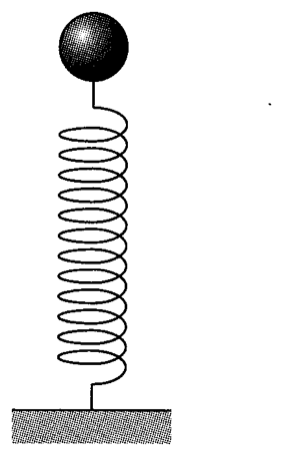
\includegraphics[keepaspectratio,width=20mm]{fig/ch3_p8_19a.png}
\end{minipage}\hfill
\begin{minipage}[t]{0.22\linewidth}
(2)\par\centering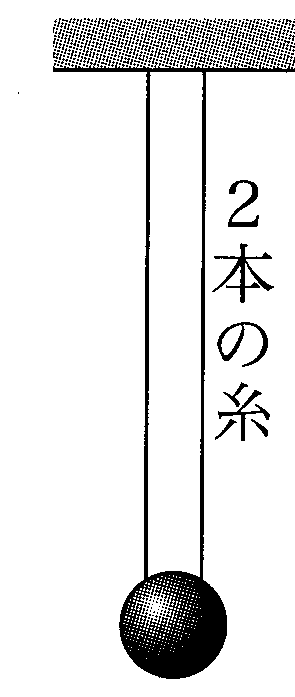
\includegraphics[keepaspectratio,width=14mm]{fig/ch3_p8_19b.png}
\end{minipage}\hfill
\begin{minipage}[t]{0.38\linewidth}
(3)\par\centering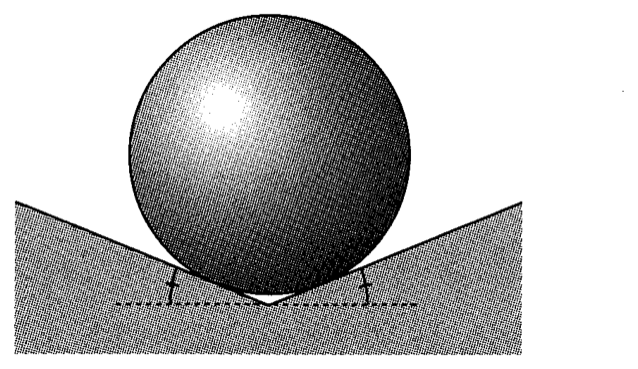
\includegraphics[keepaspectratio,width=45mm]{fig/ch3_p8_19c.png}
\end{minipage}
\end{center}

\Mon{基本事項の確認}

\begin{zuright}{43mm}
\hspace{1zw}机の上に板$\mathrm{B}$を置き，その上に物体$\mathrm{A}$を乗せる．次の力のうちで，
\begin{komon}
\ko{1} つり合いの関係にある力の組み合わせをすべて挙げよ．
\ko{2} 互いに作用・反作用の関係にある力の組み合わせをすべて挙げよ．
\end{komon}
\zusep
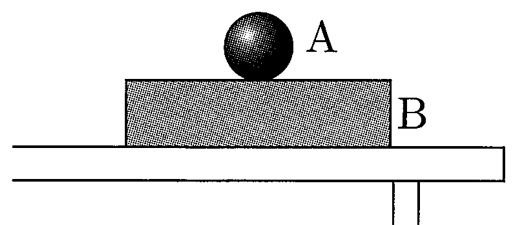
\includegraphics[keepaspectratio,width=36.5mm]{fig/ch3_p8_20.png}
\end{zuright}
\noindent\begin{tabular}{@{}p{0.49\linewidth}@{}p{0.49\linewidth}@{}}
\MARU{1}\quad 板$\mathrm{B}$が物体$\mathrm{A}$を押す力 &
\MARU{2}\quad 物体$\mathrm{A}$が板$\mathrm{B}$を押す力 \\
\MARU{3}\quad 板$\mathrm{B}$が机を押す力 &
\MARU{4}\quad 地球が物体$\mathrm{A}$を引く力 \\
\MARU{5}\quad 机が板$\mathrm{B}$を押す力 &
\MARU{6}\quad 地球が板$\mathrm{B}$を引く力 \\
\MARU{7}\quad 机が物体$\mathrm{A}$を押す力 &
\end{tabular}

\Rank{B問題}

\Mon{力のつり合い}

\begin{zuright}{62mm}
\hspace{1zw}右図のように，天井の2点$\mathrm{A}$，$\mathrm{B}$から糸$\mathrm{AC}$，$\mathrm{BC}$をぶら下げて質量$m\U{kg}$の物体をつり下げたところ，鉛直方向とそれぞれ$45^\circ$，$60^\circ$の角をなしてつり合った．このとき糸$\mathrm{AC}$，$\mathrm{BC}$の張力の大きさ$T_1$，$T_2$を求めよ．ただし，重力加速度の大きさを$g\U{m/s^2}$とする．
\zusep
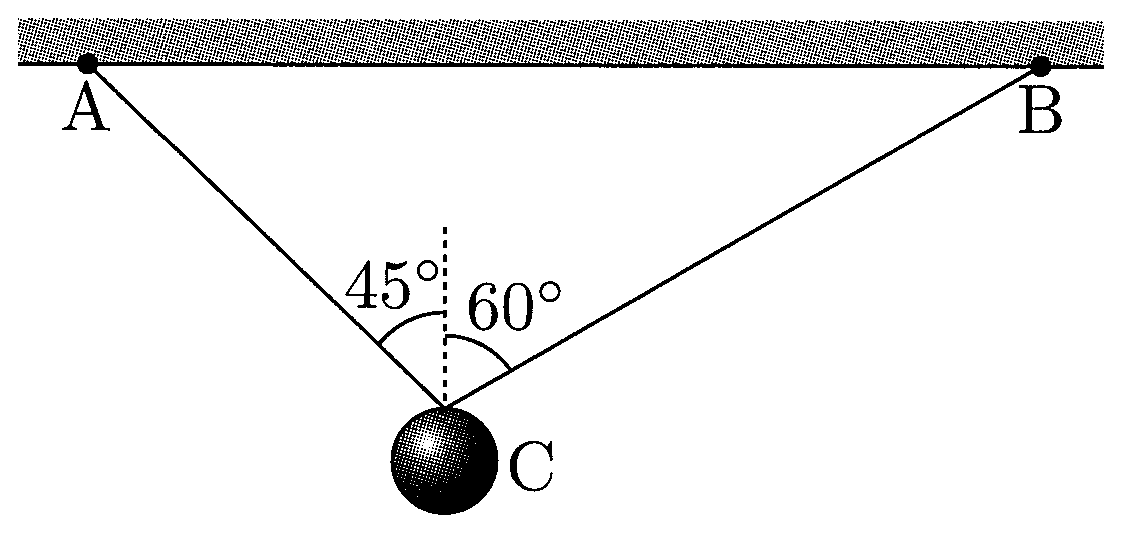
\includegraphics[keepaspectratio,width=51mm]{fig/ch3_p8_21.png}
\end{zuright}

\Mon{弾性力}\Sitei

\begin{zuright}{22mm}
\hspace{1zw}右図のように，質量が$m_1\U{kg}$のおもり$\mathrm{A}$と，質量が$m_2\U{kg}$のおもり$\mathrm{B}$を軽い糸と弾性定数$k\U{N/m}$の軽いばねでつるしたところ，ばねがある長さだけ伸びて各物体はつり合って静止した．重力加速度の大きさを$g\U{m/s^2}$として，以下の問いに答えよ．
\begin{komon}
\ko{1} 糸の張力の大きさを求めよ．
\ko{2} ばねの伸びを求めよ．
\end{komon}
\zusep
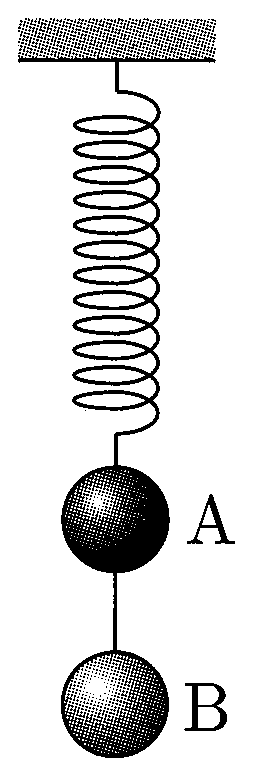
\includegraphics[keepaspectratio,width=12mm]{fig/ch3_p8_22.png}
\end{zuright}

\Mon{斜面上での最大摩擦力}

\begin{zuright}{52mm}
\hspace{1zw}右図のように，粗い面を持つ水平な板の上に質量$2.0\U{kg}$の物体を置き，水平方向に外力を加えたところ，外力が$8.0\U{N}$を越えると物体は板の上をすべり出した．重力加速度の大きさを$9.8\U{m/s^2}$として，以下の問いに有効数字2桁で答えよ．
\begin{komon}
\ko{1} 物体と板の間の静止摩擦係数を求めよ．
\ko{2} 板の上にこの物体を置いて，板を静かに傾けていく．物体がすべり始めるときの板の傾きを$\theta\U{rad}$とするとき，$\tan\theta$の値を求めよ．
\end{komon}
\zusep
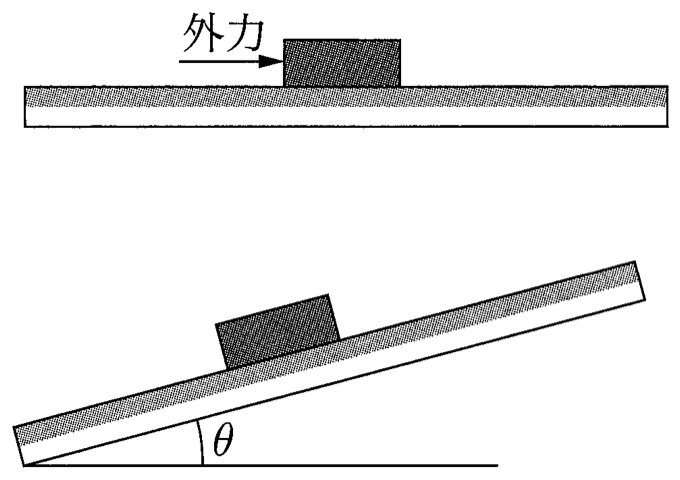
\includegraphics[keepaspectratio,width=48mm]{fig/ch3_p9_23.png}
\end{zuright}

\Mon{作用・反作用}

\begin{zuright}{35mm}
\hspace{1zw}次の文の空欄を適当な語句で埋めよ．

\hspace{1zw}台ばかりに物体$\mathrm{P}$をのせて質量を計ることができるのはなぜかを考えてみよう．重力加速度の大きさを$g\U{m/s^2}$，物体$\mathrm{P}$の質量を$m\U{kg}$とする．\MARU{3}\MARU{6}\MARU{7}は式で，その他は言葉で答えよ．

\hspace{1zw}物体$\mathrm{P}$には重力と\fbox{\MARU{1}}が作用しているが，物体$\mathrm{P}$が静止しているときにはこの二つの力は\fbox{\MARU{2}}の関係にあるので，\fbox{\MARU{1}}の大きさは\fbox{\MARU{3}}になる．

\hspace{1zw}さて，台ばかりの内部は図のように鉛直に取り付けられたバネの上に皿が乗っている構造になっており，前面の針はバネの縮みに応じて回転する仕組みになっている．台ばかりの皿は軽く，その質量を無視してよいものとして，皿に作用する力を考えると，皿にはバネからの弾性力と，\fbox{\MARU{1}}の\fbox{\MARU{4}}の関係にある力である\fbox{\MARU{5}}が作用する．そのため，この力によってバネは押し縮められる．弾性定数を$k\U{N/m}$，バネの縮みを$x\U{m}$とすると，皿に作用する力のつり合いの式は\fbox{\MARU{6}}となり，これからバネの縮みは\fbox{\MARU{7}}となる．よって，台ばかりの内部のバネの縮みの距離から，皿の上に乗っている物体の質量$m\U{kg}$を逆算することができる．
\zusep
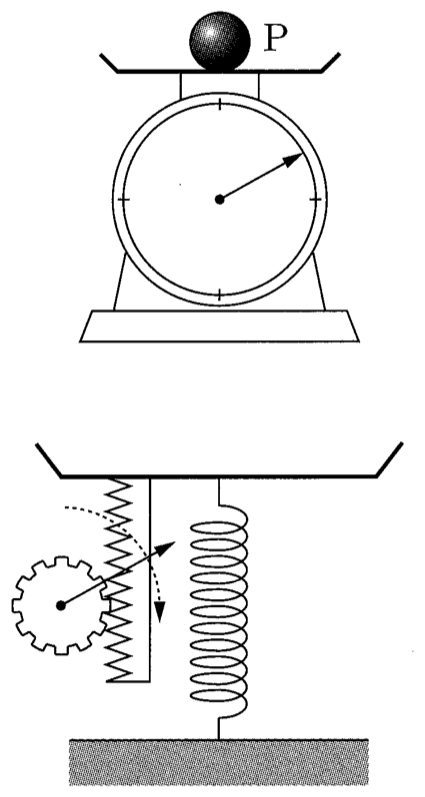
\includegraphics[keepaspectratio,width=30mm]{fig/ch3_p9_24.png}
\end{zuright}

\Mon{力のつり合い}\Sitei

\begin{zuright}{47mm}
\hspace{1zw}右図のように，仰角$30^\circ$のなめらかな斜面上に，天井から糸でつるした質量$m\U{kg}$の物体を置いたところ，糸が鉛直方向と$30^\circ$の角をなしてつり合った．糸の張力と，斜面から物体に作用する垂直抗力の大きさを求めよ．ただし，重力加速度の大きさを$g\U{m/s^2}$とする．
\zusep
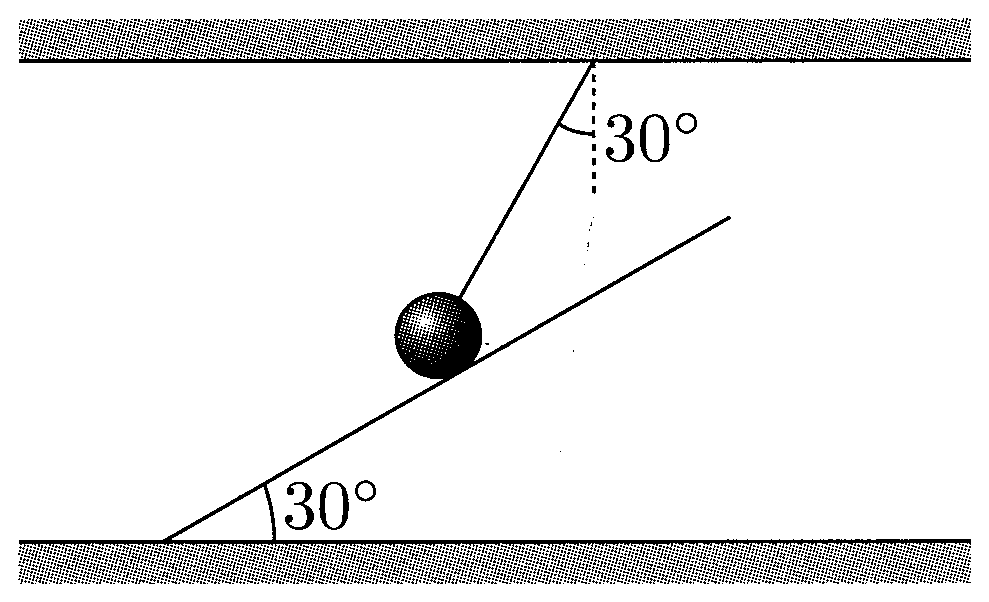
\includegraphics[keepaspectratio,width=47mm]{fig/ch3_p9_25.png}
\end{zuright}

\filbreak
\Rank{C問題}

\begingroup
\let\filbreak\relax
\Mon{弾性力}
\endgroup

\begin{zuright}{47mm}
\hspace{1zw}右図のように，自然長が$l\U{m}$でばね定数の等しいばね2本を，距離$2l\U{m}$だけ離して天井にとりつけ，2つのばねの下端をつないだ．2つのばねの先に，質量$m\U{kg}$のおもり$\mathrm{A}$をつないだところ，ばねは鉛直線と$45^\circ$の角をなしてつり合った．次に，質量$M\U{kg}$のおもり$\mathrm{B}$をつないだところ，ばねは鉛直線と$30^\circ$の角をなしてつり合った．$\mathrm{A}$と$\mathrm{B}$のおもりの質量の比$\dfrac{m}{M}$を求めよ．
\zusep
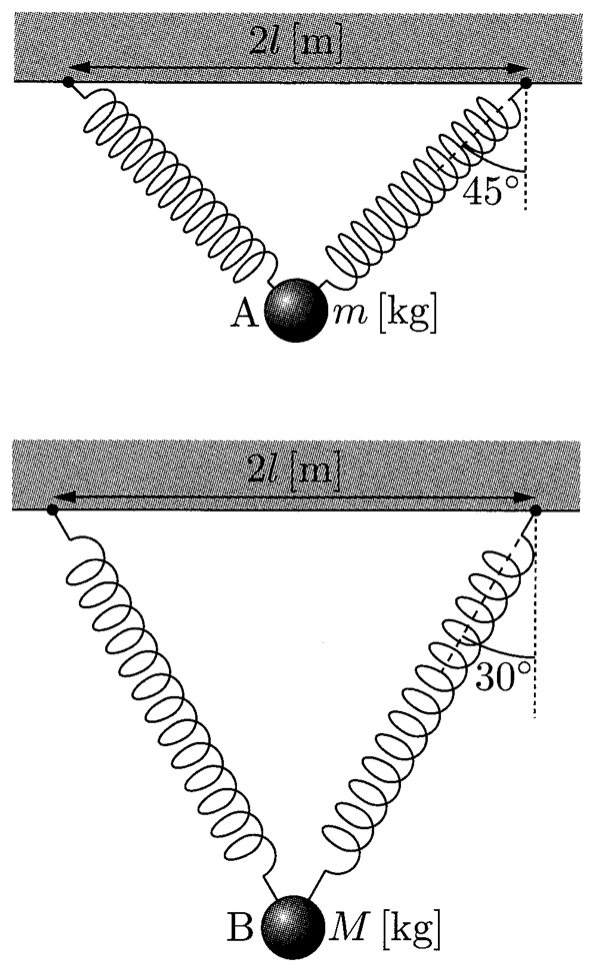
\includegraphics[keepaspectratio,width=42mm]{fig/ch3_p10_26.png}
\end{zuright}

\Mon{斜面上での最大摩擦力}

\begin{zuright}{47mm}
\hspace{1zw}右図のように，摩擦のある平板上に質量$m\U{kg}$の小物体が置かれている．重力加速度の大きさを$g\U{m/s^2}$として以下の問いに答えよ．
\begin{komon}
\ko{1} 板を静かに傾けていくと，板が水平面と角$\alpha_0$をなしたときに物体は滑り始めた．このことから，板と物体の間の静止摩擦係数$\mu_0$を$\alpha_0$で表せ．
\ko{2} 傾斜角を増して$\alpha\ (\alpha>\alpha_0)$にするとき物体が滑るのを防ぐためには，板面に平行上向きにどれだけの力を加えればよいか．その最小の力を求めよ．
\end{komon}
\zusep
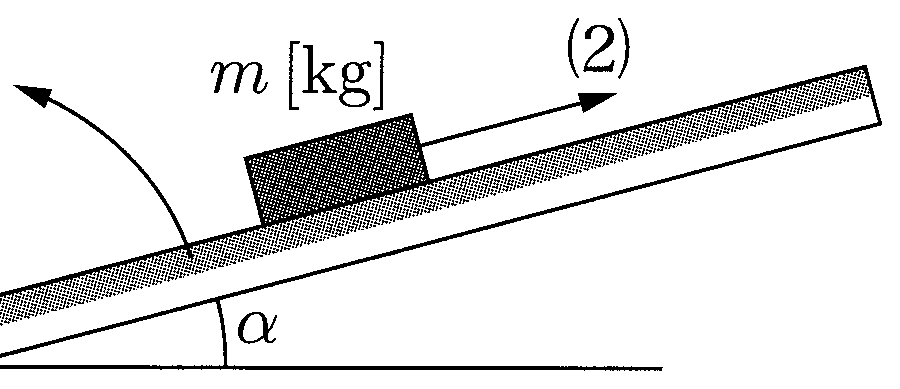
\includegraphics[keepaspectratio,width=42mm]{fig/ch3_p10_27.png}
\end{zuright}

\newpage
%%%%%%%%%%%%%%%%%%%%  解答（旧 prob_p72_2.png〜prob_p76_1.png）  %%%%%%%%%%%%%%%%%%%%
\KaiTitle{第3回　物体に作用する力とつり合い}
\setlength{\columnseprule}{0.4pt}
\begin{multicols}{2}
\raggedcolumns


\Rank{A問題}
\MonN{19}{基本事項の確認}\par\nopagebreak
\begin{sisin}
\hspace{1zw}物体に作用する力は，場の力，接触力，作用・反作用の順番に考えていくとよい．なお，場の力である重力は，地球が物体を引く力であるから作用主は地球である．
\end{sisin}
\KaiHead
\begin{zuright}{24mm}
\begin{komon}
\ko{1} 重力$W$\\
ばねが物体に及ぼす弾性力$F$
\end{komon}
\zusep
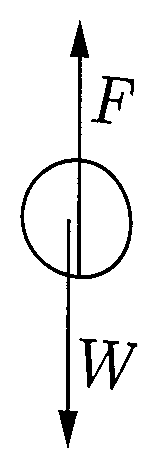
\includegraphics[keepaspectratio,height=26mm]{fig/ch3_p72_19a.png}
\end{zuright}
\begin{zuright}{28mm}
\begin{komon}
\ko{2} 重力$W$\\
右の糸が物体に及ぼす張力$T_1$\\
左の糸が物体に及ぼす張力$T_2$
\end{komon}
\zusep
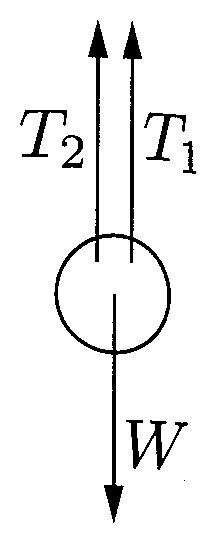
\includegraphics[keepaspectratio,height=30mm]{fig/ch3_p72_19b.png}
\end{zuright}
\begin{zuright}{32mm}
\begin{komon}
\ko{3} 重力$W$\\
右の斜面が物体に及ぼす垂直抗力$N_1$\\
左の斜面が物体に及ぼす垂直抗力$N_2$
\end{komon}
\zusep
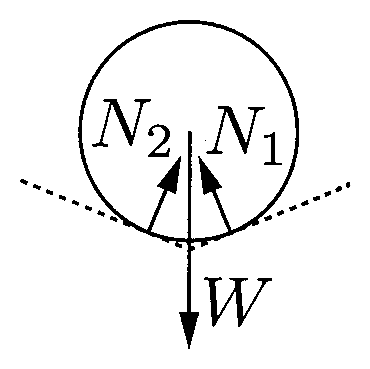
\includegraphics[keepaspectratio,width=28mm]{fig/ch3_p72_19c.png}
\end{zuright}

\MonN{20}{基本事項の確認}\par\nopagebreak
\begin{sisin}
\hspace{1zw}力のつり合いと，作用・反作用の関係とは異なるものであることに注意せよ．力のつり合いとは，\underline{ある一つ}\hskip0pt\underline{の物体に}\hskip0pt\underline{作用する}\hskip0pt\underline{いくつか}\hskip0pt\underline{の力が}\hskip0pt\underline{互いに}\hskip0pt\underline{打ち消し}\hskip0pt\underline{合っている}ことを言い，作用・反作用の関係とは，\underline{二つの}\hskip0pt\underline{物体が}\hskip0pt\underline{互いに}\hskip0pt\underline{及ぼし}\hskip0pt\underline{合っている}\hskip0pt\underline{等大・}\hskip0pt\underline{逆向きの力}のことを言う．単純に大きさだけを見て，これが同じだからつり合いとしたり，作用・反作用であるとはしないこと．また，接触力は互いに接触していなければ作用しないので，\MARU{7}の力は存在しない．

\hspace{1zw}存在する力を「$\mathrm{A}$が$\mathrm{B}$に及ぼす○○力」と正しく言って考えると分かりやすい．つりあいの関係になるのは，「$\mathrm{B}$に」の部分が共通する複数の力である．また，作用・反作用の関係になる力は「$\mathrm{A}$が$\mathrm{B}$に」の部分が「$\mathrm{B}$が$\mathrm{A}$に」となる一組の力である．
\end{sisin}
\KaiHead
\hspace{1zw}力の作用図は次図のようになる．
\begin{center}
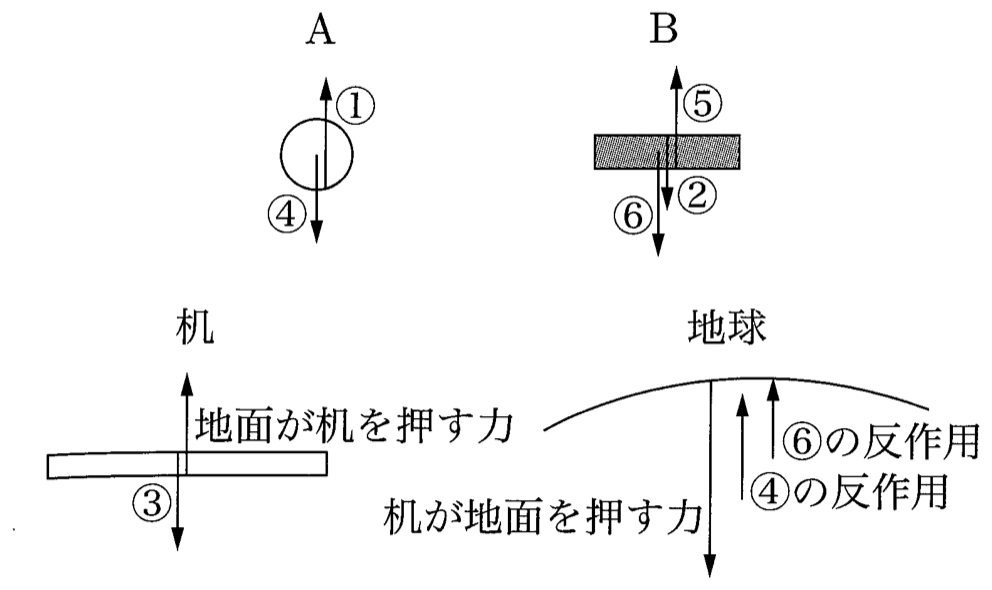
\includegraphics[keepaspectratio,width=70mm]{fig/ch3_p73_20.png}
\end{center}
\begin{komon}
\ko{1} つり合いの関係

物体$\mathrm{A}$に関して，鉛直下向きに作用する\MARU{4}と鉛直上向きに作用する\MARU{1}の力がつり合う．

板$\mathrm{B}$に関して，鉛直下向きに作用する\MARU{2}＋\MARU{6}と鉛直上向きに作用する\MARU{5}の力がつり合う．
\ko{2} 作用・反作用の関係

$\mathrm{A}$と$\mathrm{B}$間でやり取りされる垂直抗力\MARU{1}と\MARU{2}が，また$\mathrm{B}$と机間でやり取りされる垂直抗力\MARU{3}と\MARU{5}とが互いに作用・反作用の関係にある．
\end{komon}

\Rank{B問題}
\MonN{21}{力のつり合い}\par\nopagebreak
\begin{sisin}
\hspace{1zw}まず，物体に作用する力を，場の力，接触力，作用・反作用の力の順に描き出す．物体が静止している場合には描き出した力の作用図をもとにつり合い条件を考えればよい．

\hspace{1zw}力のつり合い条件のとらえ方はベクトル的に考える方法，成分分解する方法とがあるが，本問の場合は糸が2本あり，ある特殊な方向というのは考えにくい．そこで，オーソドックスに水平方向・鉛直方向に力を成分分解して，各軸方向の力のつり合いを考える．
\end{sisin}
\KaiHead
\hspace{1zw}物体に働く力の作用図は次図の通り．
\begin{center}
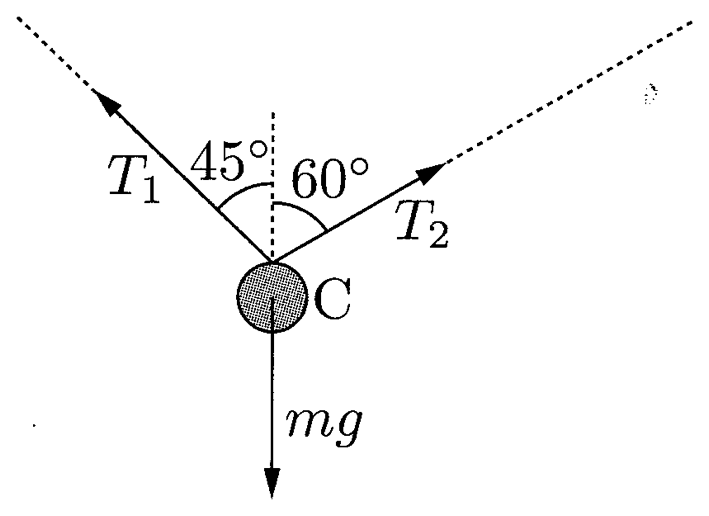
\includegraphics[keepaspectratio,width=50mm]{fig/ch3_p73_21.png}
\end{center}
\hspace{1zw}鉛直方向・水平方向のつり合いの式は，
\[
\text{鉛直方向：}\quad T_1\cos45^\circ+T_2\cos60^\circ=mg
\]
\[
\text{水平方向：}\quad T_1\sin45^\circ=T_2\sin60^\circ
\]
以上2式より，
\[
T_1=\dfrac{\sqrt2}{2}\left(3-\sqrt3\right)mg\U{N}
\]
\[
T_2=\left(\sqrt3-1\right)mg\U{N}\Ans
\]

\MonN{22}{弾性力}\par\nopagebreak
\begin{sisin}
\hspace{1zw}まず作用している力を書き出す必要がある．\underline{どの}\hskip0pt\underline{物体}\hskip0pt\underline{に対}\hskip0pt\underline{して}\hskip0pt\underline{力が}\hskip0pt\underline{作用}\hskip0pt\underline{する}\hskip0pt\underline{かに}\hskip0pt\underline{注意}\hskip0pt\underline{せよ}．物体$\mathrm{A}$については場の力として重力$m_1g$，接触力としてバネから弾性力$kx$，糸から張力$T$を受けるが，物体$\mathrm{B}$については場の力として重力$m_2g$と接触力の張力$T$の\underline{二つのみ}である．物体$\mathrm{B}$には糸しか接触しておらず，バネは接触していないから弾性力$kx$は$\mathrm{B}$には作用しない．

\hspace{1zw}同様に，各物体に対しての力のつり合いを考える際には，\underline{他の物体}\hskip0pt\underline{に作用する}\hskip0pt\underline{力を含め}\hskip0pt\underline{ては}\hskip0pt\underline{ならない}．すなわち，$\mathrm{B}$に関する力のつり合いを考えるときに$\mathrm{A}$に作用する弾性力$kx$を考えてはならないし，また$\mathrm{A}$に関する力のつり合いを考えるときに$\mathrm{B}$に作用する重力$m_2g$を含めてはならない．
\end{sisin}
\KaiHead
\begin{komon}
\ko{1} ばねののびを$x\U{m}$，糸の張力の大きさを$T\U{N}$とする．$\mathrm{A}$，$\mathrm{B}$に作用する力の作用図は次図の通りとなる．
\begin{center}
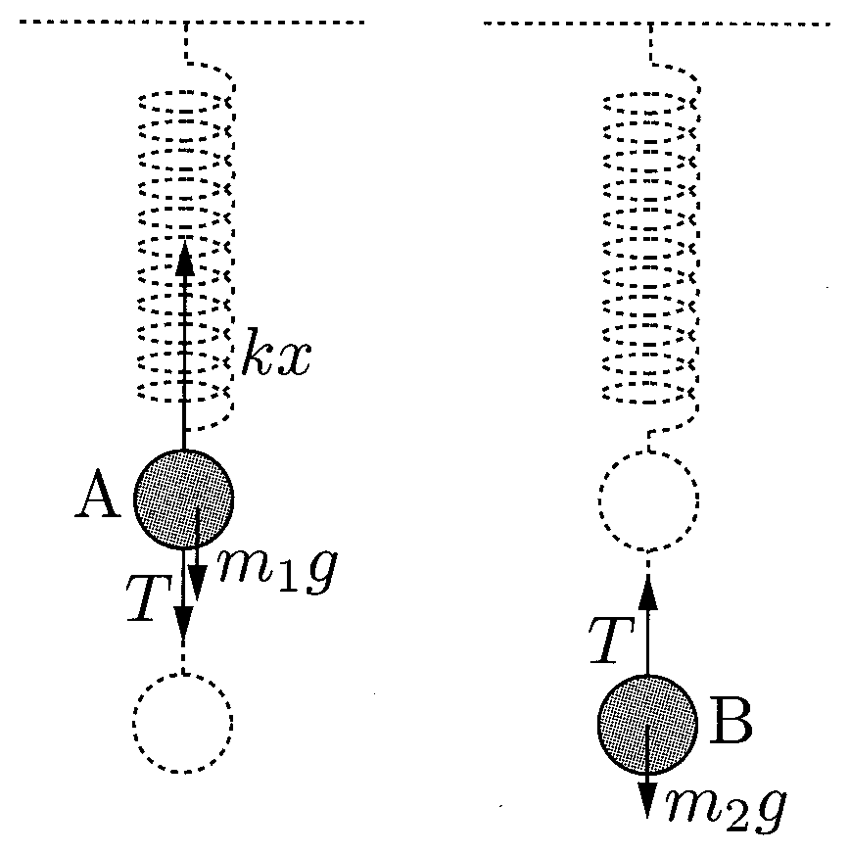
\includegraphics[keepaspectratio,width=60mm]{fig/ch3_p73_22.png}
\end{center}

よって，各物体の鉛直方向の力のつり合いの式は，
\[
\mathrm{A}:kx=m_1g+T
\]
\[
\mathrm{B}:T=m_2g
\]
以上2式より，
\[
T=m_2g\U{N}\Ans
\]
\ko{2} また，$x$については，
\[
x=\dfrac{(m_1+m_2)g}{k}\U{m}\Ans
\]
\end{komon}

\MonN{23}{斜面上での最大摩擦力}\par\nopagebreak
\begin{sisin}
\hbadness=10000
\hspace{1zw}まず，各物体に作用する力を書き出して力のつり合い条件を考えよ．\underline{静止}\hskip0pt\underline{摩擦}\hskip0pt\underline{力お}\hskip0pt\underline{よび}\hskip0pt\underline{垂直}\hskip0pt\underline{抗力}\hskip0pt\underline{の大}\hskip0pt\underline{きさ}\hskip0pt\underline{は力}\hskip0pt\underline{のつ}\hskip0pt\underline{り合}\hskip0pt\underline{いの}\hskip0pt\underline{条件}\hskip0pt\underline{式か}\hskip0pt\underline{ら決}\hskip0pt\underline{まる}ことに注意．静止摩擦力の大きさは$\mu_0N$とは限らない．本問のように，滑り出すギリギリのときには作用する静止摩擦力は最大摩擦力$\mu_0N$となるが，最初から$\mu_0N$とはおかずに，まず静止摩擦力を$f$とおき，つり合いの条件から$f$を求めて考えること．

\hspace{1zw}また，斜面上の物体のつり合いは斜面に対して平行な方向とそれに垂直な方向に力を分解して考える．
\end{sisin}
\KaiHead
\hspace{1zw}板が物体に及ぼす垂直抗力の大きさを$N\U{N}$，静止摩擦力の大きさを$f\U{N}$とする．また物体と面との間の静止摩擦係数を$\mu_0$とする．
\begin{komon}
\ko{1} 水平方向に加える外力の大きさを$F\U{N}$とするとき，物体をつり合わせるために静止摩擦力はこの外力と逆向きに作用する．ゆえに，このとき物体に働く力の作用図は次図の通り．
\begin{center}
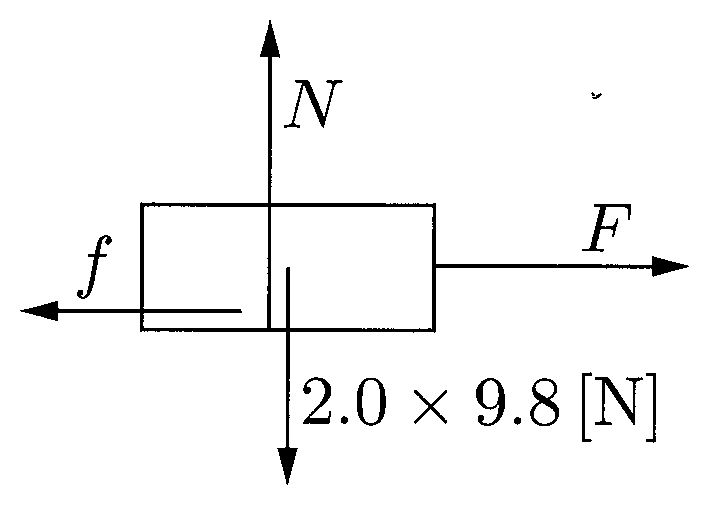
\includegraphics[keepaspectratio,width=55mm]{fig/ch3_p74_23a.png}
\end{center}

ここで，力のつり合いの条件より，
\[
\text{水平方向：}\quad f=F
\]
\[
\text{鉛直方向：}\quad N=2.0\times9.8\U{N}
\]
静止摩擦力の性質より，$f>\mu_0N=\mu_0\cdot19.6\U{N}$となると物体は滑り出すが，滑り出す瞬間の外力$F$が$8.0\U{N}$であったことから，
\[
8.0=\mu_0\cdot19.6\U{N}
\]
が成立する．よって，静止摩擦係数は
\[
\mu_0=0.408\fallingdotseq0.41\Ans
\]
\ko{2} 斜面の傾斜角が$\varphi$のときについて考える．重力の斜面方向分力$mg\sin\varphi=19.6\sin\varphi$が斜面に沿って下向きに作用して物体を滑らせようとするので，物体に作用する静止摩擦力は斜面に沿って上向きである．よって，物体に作用する力は次図の通り．
\begin{center}
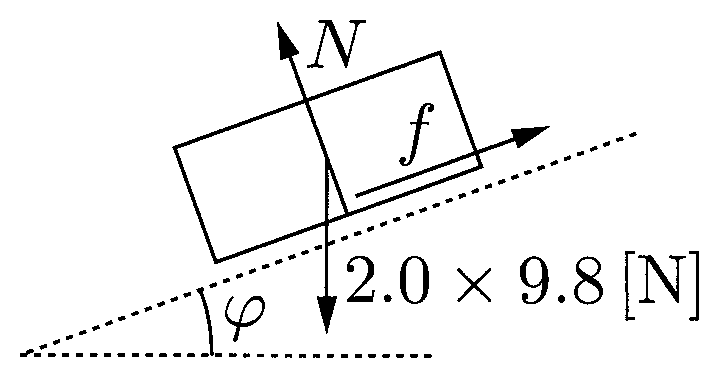
\includegraphics[keepaspectratio,width=55mm]{fig/ch3_p74_23b.png}
\end{center}

ここで，力のつり合いの条件より，
\[
\text{斜面に平行：}\quad 2\times9.8\sin\varphi=f
\]
\[
\text{斜面に垂直：}\quad N=2\times9.8\cos\varphi
\]
ゆえに，
\[
f=19.6\sin\varphi\U{N}
\]
となるが，傾斜角$\varphi$を増していくと静止しつづけるために必要な静止摩擦力は増加していき，
\[
f=\mu_0N
\]
となった直後に滑り出してしまう．その限界の角度が$\theta$であることから，
\[
19.6\sin\theta=0.408\times19.6\cos\theta
\]
整理して，
\[
\tan\theta=0.408\fallingdotseq0.41\Ans
\]
\end{komon}

\MonN{24}{作用・反作用}\par\nopagebreak
\begin{sisin}
\hspace{1zw}物体$\mathrm{P}$と台ばかりにそれぞれ着目して力の作用図を描く．うまく誘導に沿って考えよう．

\hspace{1zw}「力」についての説明を求められたら，「○○が△△に対して及ぼす××力」という形式で答えよう．何が何に対して及ぼしている力なのかを明確にすること．
\end{sisin}
\KaiHead
\hspace{1zw}物体$\mathrm{P}$および台ばかりの皿について力の作用図を描くと次図の通りとなる．
\begin{center}
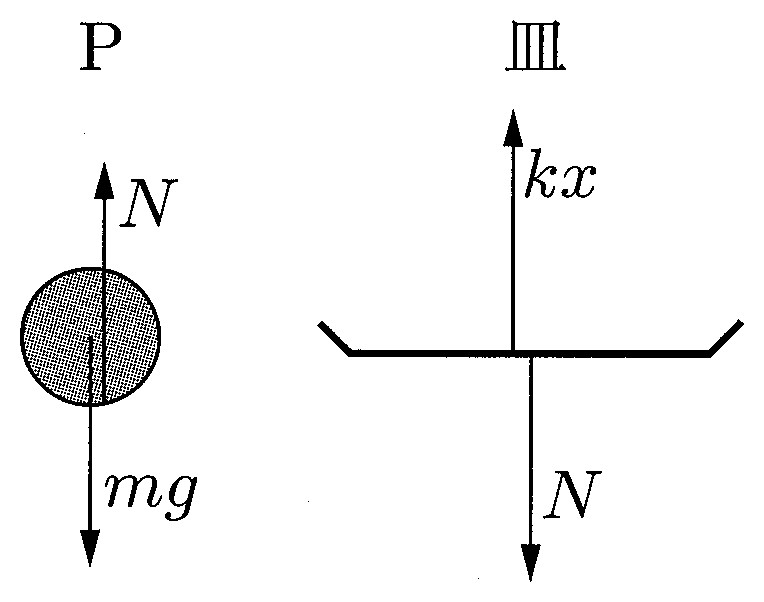
\includegraphics[keepaspectratio,width=60mm]{fig/ch3_p74_24.png}
\end{center}
\hspace{1zw}よって，
\begin{description}
\item[\MARU{1}] 皿が物体$\mathrm{P}$に及ぼす垂直抗力
\item[\MARU{2}] つり合い
\item[\MARU{3}] $mg\U{N}$
\item[\MARU{4}] 作用・反作用
\item[\MARU{5}] 物体$\mathrm{P}$が皿に及ぼす垂直抗力
\item[\MARU{6}] $kx=mg$
\item[\MARU{7}] $x=\dfrac{mg}{k}\U{m}$
\end{description}
\begin{chuu}
\hspace{1zw}\MARU{6}の立式の右辺にある$mg$は，物体$\mathrm{P}$に作用する重力ではなく，\MARU{5}の垂直抗力を表していることに注意せよ．この\MARU{5}の力は，\MARU{2}および\MARU{4}の事項より，大きさが$mg\U{N}$になっている．

% TODO: 原本では「バネばかり」表記（台ばかりの誤りと思われる）
\hspace{1zw}また，以上のことから分かるように，バネばかりは物体の質量そのものを計っているのではなく，バネばかりの皿に対して作用する力を計っている．すなわち，バネばかりの針が$m\U{kg}$を指している場合には，バネの皿に対して大きさ$mg\U{N}$の力が下向きに作用しているということを意味している．
\end{chuu}

\MonN{25}{力のつり合い}\par\nopagebreak
\begin{sisin}
\hspace{1zw}本問のような複雑な力のつり合いの問題でも，基本は\MARU{1}「作用している力の書き出し」，\MARU{2}「力のつり合いの式の立式」の二つの手順を踏むのみである．

\hspace{1zw}「なめらかな斜面」とは摩擦のない斜面のことを意味する．
\end{sisin}
\KaiHead
\hspace{1zw}糸が物体に及ぼす張力の大きさを$T\U{N}$，斜面が物体に及ぼす垂直抗力の大きさを$N\U{N}$とすれば，物体に働く力の作用図は図の通り．
\begin{center}
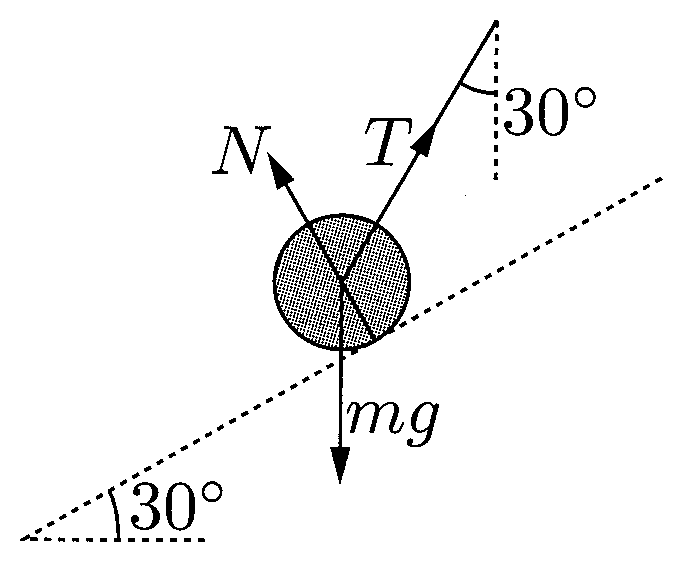
\includegraphics[keepaspectratio,width=50mm]{fig/ch3_p75_25.png}
\end{center}
\hspace{1zw}力のつり合いの式を立てると，
\[
\text{斜面に平行な方向：}\quad mg\sin30^\circ=T\cos30^\circ
\]
\[
\text{斜面に垂直な方向：}\quad N+T\sin30^\circ=mg\cos30^\circ
\]
よって，
\[
T=\dfrac{\sqrt3}{3}mg\U{N},\quad N=\dfrac{\sqrt3}{3}mg\U{N}\Ans
\]
\begin{bekkai}
\hspace{1zw}水平方向・鉛直方向に力を分解して考えてもよい．次のようになり，同じ答えが得られる．
\[
\text{水平方向：}\quad N\sin30^\circ=T\sin30^\circ
\]
\[
\text{鉛直方向：}\quad N\cos30^\circ+T\cos30^\circ=mg
\]
\end{bekkai}

\Rank{C問題}
\MonN{26}{弾性力}\par\nopagebreak
\begin{sisin}
\hspace{1zw}バネが物体に作用する力は，その伸び（もしくは縮み）によって決まる．バネの全長と伸びとを混同しないように注意せよ．
\end{sisin}
\KaiHead
\hspace{1zw}弾性定数を$k\U{N/m}$，重力加速度の大きさを$g\U{m/s^2}$とする．

\noindent\underline{物体$\mathrm{A}$について}\par
\hspace{1zw}このときのバネの全長は$\sqrt2\,l$であるから，自然長から$\left(\sqrt2-1\right)l$だけ伸びている．よって，物体$\mathrm{A}$にバネが作用する弾性力はフックの法則より$\left(\sqrt2-1\right)kl\U{N}$であり，物体$\mathrm{A}$に働く力の作用図は次図の通りとなる．
\begin{center}
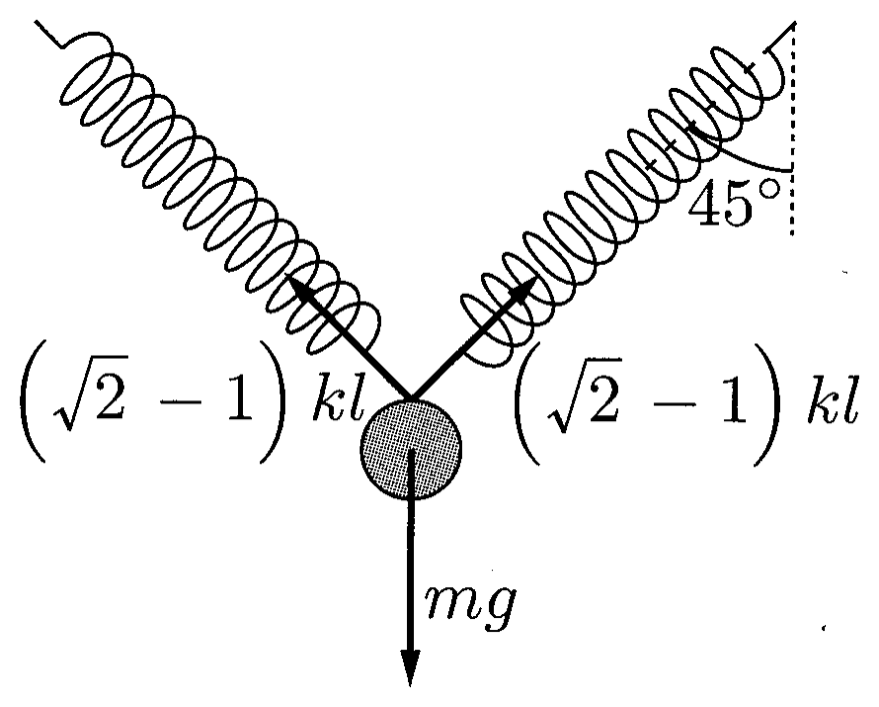
\includegraphics[keepaspectratio,width=62mm]{fig/ch3_p75_26.png}
\end{center}
\hspace{1zw}鉛直方向の力のつり合いについて，
\[
2\times\left(\sqrt2-1\right)kl\cos45^\circ=mg
\]
であるから，
\[
m=\dfrac{\left(2-\sqrt2\right)kl}{g}\U{kg}\Eq{1}
\]

\noindent\underline{物体$\mathrm{B}$について}\par
\hspace{1zw}同様に考えると，バネの全長は$2l\U{m}$なので，$\mathrm{B}$に作用する弾性力の大きさは$kl\U{N}$であり，鉛直方向の力のつり合いの式は，
\[
2\times kl\cos30^\circ=Mg
\]
よって，
\[
M=\dfrac{\sqrt3\,kl}{g}\U{kg}\Eq{2}
\]
\MARU{1}\MARU{2}より，
\[
\dfrac{m}{M}=\dfrac{2\sqrt3-\sqrt6}{3}\Ans
\]

\MonN{27}{斜面上での最大摩擦力}\par\nopagebreak
\begin{sisin}
\hspace{1zw}(1)については前出の問題と同じなのでよかろう．(2)についても基本的な考えは，力の作用図の作図，つり合いの式の立式である．問題なのは作用する静止摩擦力の向きである．この物体は重力の斜面方向分力$mg\sin\alpha$によって滑り出そうとするので，これを防ぐには静止摩擦力が上向きに作用すればよい．ところが$\alpha>\alpha_0$の場合には，物体が滑り出すのを防ぐために必要なだけの静止摩擦力を作用することができない．なるべく小さな力で物体が滑り出すのを防ぐためには，静止に必要な力を補うべく上向きに力を加えてやればよい．よって，作用している静止摩擦力は上向きと分かる．このような直観的な考え方が分かりにくい人は，静止摩擦力が下向きに作用する場合についても図を描いて立式し，考えてみよ．この場合，静止するのに必要な外力は，摩擦力が上向きに作用する場合に比べて大きくなることが計算によって示される．
\end{sisin}
\KaiHead
\hspace{1zw}物体に作用する垂直抗力の大きさを$N\U{N}$，静止摩擦力の大きさを$f\U{N}$とする．
\begin{komon}
\ko{1} 水平面との傾角が$\alpha_0$のとき，物体に働く力の作用図は次図の通り．
\begin{center}
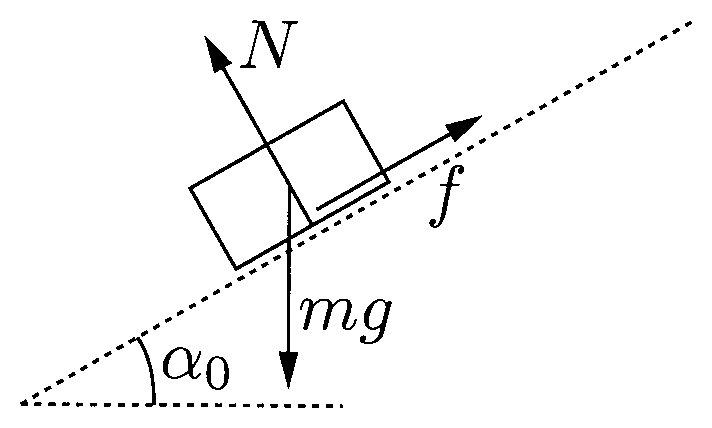
\includegraphics[keepaspectratio,width=55mm]{fig/ch3_p75_27a.png}
\end{center}

ここで，各方向の力のつり合いは，
\[
\text{斜面に平行な方向：}\quad mg\sin\alpha_0=f
\]
\[
\text{斜面に垂直な方向：}\quad N=mg\cos\alpha_0
\]
また，このとき板が物体に及ぼす静止摩擦力は最大摩擦力となっているので，
\[
f=\mu_0N
\]
以上より，
\[
\mu_0=\tan\alpha_0\Ans
\]
\ko{2} 水平面との傾角が$\alpha$のとき，物体がすべるのを防ぐために板と平行上向きに加える力の大きさを$f'$とする．このとき，物体に働く力は次図の通り．
\begin{center}
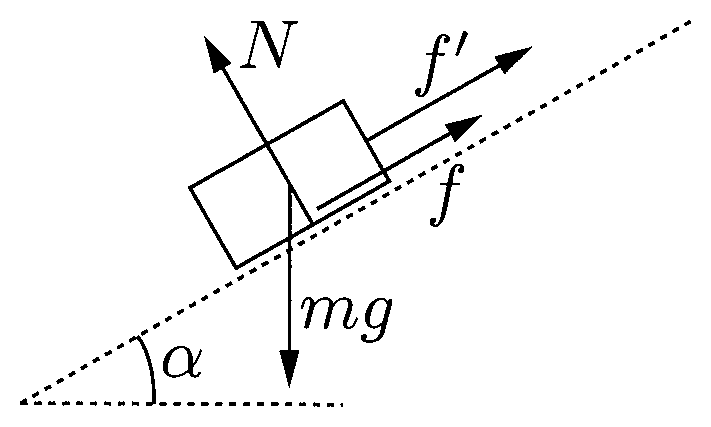
\includegraphics[keepaspectratio,width=55mm]{fig/ch3_p76_27b.png}
\end{center}

力のつり合いより，
\[
\text{斜面に平行な方向：}\quad mg\sin\alpha=f+f'
\]
% TODO: 原本ママ．「斜面に垂直な方向」の誤りと思われる
\[
\text{鉛直に垂直な方向：}\quad N=mg\cos\alpha
\]
物体が静止をしつづけるためには，作用している静止摩擦力が，最大摩擦力$\mu_0N$を越えなければよい．
\[
f\leqq\mu_0N
\]
以上の式を満たすような$f'$は，
\[
f'\geqq mg\left(\sin\alpha-\mu_0\cos\alpha\right)
\]
である．よって，加えるべき最小限の力の大きさは，これに(1)の答えを代入して
\[
mg\left(\sin\alpha-\tan\alpha_0\cos\alpha\right)\U{N}\Ans
\]
\end{komon}
\begin{bsHosoku}{参考}
\hspace{1zw}物体に加える力$f'$を大きくしていくと，いずれ物体は斜面にそって上向きに動き出す．動き始める瞬間の$f'$の大きさを求めてみよう．

\hspace{1zw}静止摩擦力の向きに注意すると，動き始める瞬間の力のつりあいの式は次のようになる．
\[
\text{斜面に平行な方向：}\quad mg\sin\alpha+f=f'
\]
% TODO: 原本ママ．「斜面に垂直な方向」の誤りと思われる
\[
\text{鉛直に垂直な方向：}\quad N=mg\cos\alpha
\]
これらと$f=\mu_0N$を連立すると，
\[
f'=mg\left(\sin\alpha+\tan\alpha_0\cos\alpha\right)
\]
が分かる．これが物体を上向きに動かすのに必要な最小の力であるから，物体を斜面上に静止させておくには，斜面にそって上向きに
\[
mg\left(\sin\alpha-\mu_0\cos\alpha\right)\leqq f'
\]
\[
\hspace{8zw}\leqq mg\left(\sin\alpha+\tan\alpha_0\cos\alpha\right)
\]
を満たす力$f'$を加えればよい．
\end{bsHosoku}

\end{multicols}
